%versi 2 (8-10-2016) 
\chapter{Pendahuluan}
\label{chap:intro}
   
\section{Latar Belakang}
\label{sec:latar}
Dengan semakin banyaknya penambangan data yang dilakukan dan data yang digunakan juga semakin banyak, semakin banyak juga privasi di dalam data tersebut yang tersebar kepada pihak yang melakukan penambangan data. Data privasi tersebut dapat tersebar kepada pihak yang tidak bertanggung jawab dan disalahgunakan. Oleh karena itu perlu adanya suatu cara untuk mencegah privasi tersebar pada proses penambangan data, menjaga privasi pada data tersebut. Istilah untuk hal tersebut adalah \textit{privacy preserving data mining}.

Ada kesulitan dalam menentukan data seperti apa yang dapat disebut sebagai privasi. Privasi dapat dikatakan adalah sebuah informasi personal seseorang yang dapat mengidentifikasi suatu hal pada orang tersebut. Konsep yang sering kali digunakan untuk mendeskripsikan informasi personal adalah\textit{Personally Identifiable Information} yang disingkat PII. PII adalah segala informasi mengenai individu yang dikelola oleh sebuah instansi, termasuk segala informasi yang dapat digunakan untuk membedakan atau mengusut identitas seseorang dan juga segala informasi yang berhubungan atau dapat dihubungkan kepada suatu individu, seperti informasi medis, pendidikan, finansial, dan pekerjaan seseorang. 

Salah satu cara untuk melakukan \textit{privacy preserving data mining} adalah dengan melakukan modifikasi data yang ada sebelum diberikan kepada pihak lain. Ada macam-macam teknik dan algoritma yang bertujuan modifikasi data untuk \textit{privacy preserving data mining}, dibagi menjadi dua jenis yaitu \textit{Perturbation Approach} dan \textit{Anonymization Approach}. \textit{Perturbation Approach} adalah pendekatan untuk \textit{privacy preserving data mining} dengan cara mengacaukan data yang ada, tetapi hasil data yang dikacaukan masih tetap dapat ditambang. \textit{Perturbation Approach} dapat dibagi menjadi dua jenis yaitu \textit{Value-based Perturbation Techniques} dan \textit{Multi-Dimensional Perturbation}.

\begin{figure}
	\centering
	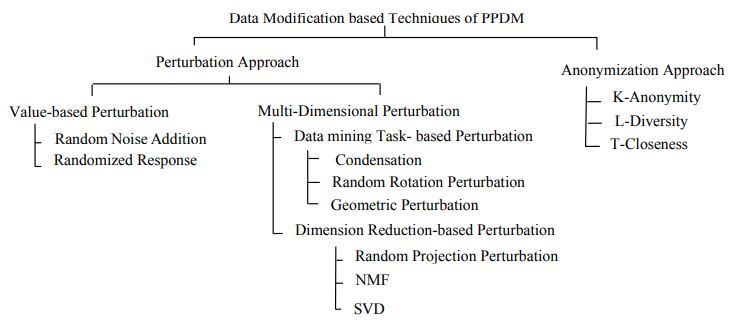
\includegraphics[scale=0.56]{ppdm}
	\caption{Berbagai macam teknik modifikasi data untuk \textit{privacy preserving data mining}}
	\label{fig:ppdm}
\end{figure}

\textit{Value-based Perturbation Techniques} adalah teknik yang bekerja dengan cara menyisipkan \textit{random noise} pada data. Sedangkan terdapat dua jenis teknik \textit{Multi-Dimensional Perturbation} yaitu \textit{Data mining Task-based Perturbation} dan \textit{Dimension Reduction-based Perturbation}. \textit{Data mining Task-based Perturbation} adalah teknik yang bekerja dengan cara modifikasi data sehingga properti yang bertahan pada data yang telah dimodifikasi spesifik hanya properti yang digunakan oleh suatu teknik penambangan data tertentu. Sedangkan \textit{Dimension Reduction-based Perturbation} adalah teknik yang bekerja dengan cara modifikasi data sekaligus mengurangi dimensi dari data asli.

Dari berbagai macam teknik modifikasi data untuk \textit{privacy preserving data mining} yang dapat dilihat pada Gambar~\ref{fig:ppdm}, terdapat empat teknik yang menggunakan metode \textit{Randomization} yaitu \textit{Random Noise Addition}, \textit{Randomized Response}, \textit{Random Rotation Perturbation}, dan \textit{Random Projection Perturbation}.

Pada penelitian ini, akan dibuat sebuah perangkat lunak yang dapat memproses data yang akan ditambang menjadi data yang telah dimodifikasi dengan metode \textit{Randomization} sehingga privasi pada data tersebut terlindungi, tetapi masih dapat ditambang. Dari berbagai macam teknik dengan metode \textit{Randomization} yang ada, dipilih dua buah teknik yaitu \textit{Random Rotation Perturbation} dan \textit{Random Projection Perturbation} untuk diimplementasikan pada perangkat lunak serta membandingkan hasil dari kedua teknik tersebut.

\section{Rumusan Masalah}
\label{sec:rumusan}
Berdasarkan latar belakang, rumusan masalah pada penelitian ini adalah sebagai berikut.
\begin{enumerate}
	\item Bagaimana cara kerja teknik \textit{Random Rotation Perturbation} dan \textit{Random Projection Perturbation} untuk \textit{privacy preserving data mining}?
	\item Bagaimana implementasi dari teknik \textit{Random Rotation Perturbation} dan \textit{Random Projection Perturbation} pada perangkat lunak?
	\item Bagaimana perbandingan antara hasil dari teknik \textit{Random Rotation Perturbation} dan \textit{Random Projection Perturbation}?
\end{enumerate}

\section{Tujuan}
\label{sec:tujuan}
Berdasarkan rumusan masalah, maka tujuan dari penelitian ini adalah sebagai berikut.
\begin{enumerate}
	\item Mempelajari cara kerja dari teknik \textit{Random Rotation Perturbation} dan \textit{Random Projection Perturbation} untuk \textit{privacy preserving data mining}
	\item Mengimplementasikan teknik \textit{Random Rotation Perturbation} dan \textit{Random Projection Perturbation} pada perangkat lunak
	\item Melakukan analisis dan pengujian untuk membandingkan dan mengukur hasil dari teknik \textit{Random Rotation Perturbation} dan \textit{Random Projection Perturbation}
\end{enumerate}

\section{Batasan Masalah}
\label{sec:batasan}
Batasan-batasan masalah untuk penelitian ini adalah sebagai berikut.
\begin{enumerate}
    \item Penelitian ini menguji apakah dataset yang telah diacak dapat digunakan untuk penambangan data dan menghasilkan kualitas yang sama atau mendekati aslinya
    \item Penelitian ini tidak menguji kualitas privasi yang hilang atau seberapa kuat dataset yang telah diacak dapat dikembalikan ke aslinya
    \item Penelitian ini hanya menguji dengan teknik penambangan data tertentu dan dengan metode tertentu
    \item Penelitian ini hanya menggunakan data yang bersifat numerik
\end{enumerate}

\section{Metodologi}
\label{sec:metlit}
Metodologi yang digunakan dalam penelitian ini adalah sebagai berikut.
\begin{enumerate}
    \item Melakukan studi literatur dasar-dasar privasi data
    \item Melakukan studi literatur teknik \textit{Random Rotation Perturbation} dan \textit{Random Projection Perturbation} untuk \textit{privacy preserving data mining}
    \item Melakukan studi literatur teknik penambangan data yang akan digunakan
    \item Melakukan analisis terhadap teknik \textit{Random Rotation Perturbation} dan \textit{Random Projection Perturbation} serta bagaimana penerapannya dengan teknik penambangan data yang akan digunakan
    \item Melakukan perancangan perangkat lunak yang mengimplementasikan teknik \textit{Random Rotation Perturbation} dan \textit{Random Projection Perturbation}
    \item Membangun perangkat lunak yang mengimplementasikan teknik \textit{Random Rotation Perturbation} dan \textit{Random Projection Perturbation}
    \item Menguji perangkat lunak secara fungsional dan eksperimental dengan menggunakan \textit{real} data
    \item Menerapkan teknik penambangan data terhadap data yang telah diproses untuk menganalisis hasil dari teknik \textit{Random Rotation Perturbation} dan \textit{Random Projection Perturbation}
    \item Melakukan analisis dan pengujian untuk membandingkan dan mengukur hasil dari teknik \textit{Random Rotation Perturbation} dan \textit{Random Projection Perturbation}
    \item Menarik kesimpulan berdasarkan hasil eksperiment yang telah dilakukan
\end{enumerate}

\section{Sistematika Pembahasan}
\label{sec:sispem}
Laporan penelitian tersusun ke dalam enam bab secara sistematis sebagai berikut.
\begin{itemize}
    \item Bab 1 Pendahuluan\\
    Berisi latar belakang, rumusan masalah, tujuan, batasan masalah, metodologi penelitian, dan sistematika pembahasan.
    \item Bab 2 Dasar Teori\\
    Berisi dasar teori tentang dasar-dasar privasi data, \textit{Random Rotation Perturbation}, \textit{Random Projection Perturbation}, \textit{Random Rotation Perturbation}, dan teknik penambangan data.
    \item Bab 3 Analisis\\
    Berisi analisis masalah, studi kasus, dan diagram aliran proses.
    \item Bab 4 Perancangan\\
    Berisi perancangan perangkat lunak yang dibangun meliputi perancangan antarmuka dan diagram kelas yang lengkap.
    \item Bab 5 Implementasi dan Pengujian\\
    Berisi implementasi antarmuka perangkat lunak, pengujian fungsional, pengujian eksperimental, dan kesimpulan dari pengujian.
    \item Bab 6 Kesimpulan dan Saran\\
    Berisi kesimpulan dari awal hingga akhir penelitian dan saran untuk pengembangan selanjutnya.
\end{itemize}